\documentclass[11pt,a4paper]{article}
\usepackage[margin=2.3cm]{geometry}
\usepackage{amsmath,amssymb,bm}
\usepackage{siunitx}
\usepackage{booktabs}
\usepackage{graphicx}
\usepackage{tikz}
\usetikzlibrary{arrows.meta,calc,positioning}
\usepackage{pgfplots}
\pgfplotsset{compat=1.17}
\usepackage{enumitem}
\usepackage{float}
\tikzset{capt/.style={text width=5.2cm,align=center}}
\usepackage[colorlinks=true,linkcolor=blue!60!black,urlcolor=blue!60!black]{hyperref}
\usepackage{fancyhdr}
\usepackage{tcolorbox}
\tcbuselibrary{skins,breakable}
\sisetup{per-mode=symbol,detect-all}

\newtcolorbox{keybox}[1]{colback=blue!4,colframe=blue!50!black,title=#1,fonttitle=\bfseries,breakable}
\newtcolorbox{examplebox}[1]{colback=green!4,colframe=green!40!black,title=#1,fonttitle=\bfseries,breakable}
\newtcolorbox{aerobox}[1]{colback=orange!5,colframe=orange!60!black,title=#1,fonttitle=\bfseries,breakable}

\pagestyle{fancy}
\fancyhf{}
\lhead{
\includegraphics[height=0.6cm]{logos/itu_logo_laci.pdf}\ \ UCK 364E Design of Machine Elements}
\setlength{\headheight}{20pt}
\rhead{Lecture 2 -- Notes}
\cfoot{\thepage}

\title{\textbf{UCK 364E Design of Machine Elements}\\[4pt]
\Large Lecture 2: Fatigue --- the Stress-Life and Strain-Life Approaches\\[2pt]
\large Cyclic loading, S--N curves, endurance limit, notch and surface effects, mean stress, cumulative damage, $\varepsilon$--N}
\author{Prof.\ Dr.\ Onur Tunçer\\ Department of Aeronautical Engineering, Istanbul Technical University}
\date{Fall 2026}

\begin{document}
\maketitle

\section*{Learning objectives}
By the end of this lecture you should be able to
\begin{enumerate}[nosep]
  \item describe the three stages of fatigue damage and explain why fatigue is a \emph{local}, surface-initiated phenomenon;
  \item define the quantities that describe a cycle ($\sigma_a$, $\sigma_m$, $R$, $A$) and convert between them;
  \item construct an S--N (W\"ohler) curve for a component from material data, applying the Marin modifying factors for surface, size, loading, temperature and reliability;
  \item compute the fatigue notch factor $K_f$ from $K_t$ using notch sensitivity, and explain why $K_f<K_t$;
  \item apply the Goodman, Gerber, Soderberg and Morrow mean-stress corrections and say which one aerospace practice uses;
  \item accumulate damage over a variable-amplitude spectrum with Palmgren--Miner, and count cycles with the rainflow method;
  \item explain the strain-life (Coffin--Manson) approach, Neuber's rule and when $\varepsilon$--N is required instead of S--N;
  \item relate all of the above to the safe-life philosophy of CS-25.571 and to the scatter factors used in certification.
\end{enumerate}

\section{Why fatigue governs aircraft structure}

In Lecture~1 every static margin we computed was large: the fuselage skin had an ultimate margin of 2.9, the actuator rod end 5.6. Nothing in an aircraft is sized by a single application of load. What sizes it is the \emph{repetition} of loads far below the static allowable: one pressurisation cycle per flight, a gust spectrum through every hour of cruise, a landing impact per flight, vibration from the propeller or rotor at hundreds of hertz.

\begin{keybox}{The central fact}
A metal loaded repeatedly to a stress well below its yield strength will eventually crack. There is no ``safe'' static margin that protects against this; the only protections are to keep the cyclic stress low enough, to limit the number of cycles, or to find the crack before it becomes critical.
\end{keybox}

Fatigue was the lesson of the de Havilland Comet (1954) and it remains the dominant design driver for pressurised fuselages, wing lower surfaces, lugs and fittings, and every joint. Two historical approaches to fatigue life exist and this lecture covers both:
\begin{itemize}[nosep]
  \item the \textbf{stress-life (S--N)} approach, valid when stresses stay elastic and lives are long ($N>10^{3}$--$10^{4}$ cycles), which is the workhorse for most machine elements;
  \item the \textbf{strain-life ($\varepsilon$--N)} approach, needed where local plasticity occurs at notches and lives are short, and which is the physically correct description of crack initiation.
\end{itemize}
The third approach, \textbf{fracture mechanics} (crack \emph{growth} rather than initiation), is the subject of the next lecture.

\subsection{The three stages of fatigue}
\begin{enumerate}[nosep]
  \item \textbf{Crack initiation}. Cyclic slip in favourably oriented surface grains produces intrusions and extrusions; a microcrack of the order of one grain diameter forms, almost always at a free surface and almost always at a stress concentration. In a well-finished laboratory specimen this stage can consume 90\% of the life; in a notched, corroded or poorly finished part, almost none of it.
  \item \textbf{Stable crack growth}. The crack grows a small increment per cycle, normal to the maximum principal stress, leaving \emph{striations} --- one per cycle --- and, on a macroscopic scale, \emph{beach marks} that record changes in load level. This stage is described quantitatively by fracture mechanics.
  \item \textbf{Final fracture}. The remaining section can no longer carry the peak load and fails statically, in one cycle, leaving a rough, fibrous or crystalline area.
\end{enumerate}
\begin{figure}[H]\centering

\begin{tikzpicture}[scale=1.0,>=Stealth,font=\scriptsize]
% grains
\draw[thick] (0,0) rectangle (4.6,2.2);
\foreach \x/\y in {0.9/0,2.1/0,3.4/0} \draw[gray!60] (\x,0) -- ($(\x,0)+(0.3,2.2)$);
\node[anchor=north] at (2.3,-0.05) {grains near a free surface};
% slip bands in one grain
\foreach \i in {0,...,5} \draw[blue!60!black] ({1.3+\i*0.12},2.2) -- ({1.0+\i*0.12},0.9);
% extrusion / intrusion on the surface
\draw[thick,red!70!black] (1.25,2.2) -- (1.32,2.42) -- (1.39,2.2);
\draw[thick,red!70!black] (1.60,2.2) -- (1.67,1.98) -- (1.74,2.2);
\node[anchor=west,red!70!black] at (1.95,2.45) {extrusion};
\node[anchor=west,red!70!black] at (1.95,1.95) {intrusion $\rightarrow$ microcrack};
\draw[->,red!70!black] (1.93,2.45) -- (1.40,2.40);
\draw[->,red!70!black] (1.93,1.98) -- (1.72,2.02);
\draw[<->,thick] (-0.4,0.6) -- (-0.4,1.6) node[midway,left,align=right] {cyclic\\ $\pm\sigma$};
\end{tikzpicture}

\caption{Crack nucleation. Cyclic slip in favourably oriented surface grains is irreversible: each cycle leaves a step, the steps pile up into an extrusion and its matching intrusion, and the intrusion is a notch one grain deep that the following cycles turn into a microcrack.}
\label{fig:slip}
\end{figure}

A fatigue fracture surface is therefore readable: a smooth, beach-marked region (growth) adjoining a rough region (final fracture), with the initiation site at the focus of the beach marks. Reading a fracture surface is the first step in every failure investigation.

\begin{figure}[H]\centering
\begin{tikzpicture}[scale=1.0,>=Stealth,font=\small]
\coordinate (I) at (-2.0,0);
\begin{scope}
  \clip (0,0) circle (2.0);
  \fill[blue!8] (-2.2,-2.2) rectangle (2.2,2.2);
  \foreach \r in {0.6,1.0,1.4,1.8,2.2,2.6} \draw[blue!55!black] (I) circle (\r);
  \fill[gray!45] (1.15,-2.2) rectangle (2.3,2.2);
  \draw[gray!60!black] (1.15,-2.2) -- (1.15,2.2);
  \foreach \i in {0,...,14} \draw[gray!60!black] ({1.3+0.07*rnd},{-2.1+\i*0.3}) -- ({1.9+0.2*rnd},{-1.95+\i*0.3});
\end{scope}
\draw[thick] (0,0) circle (2.0);
\fill[red] (I) circle (2.5pt);
\node[anchor=east,align=right] at (-2.35,0) {initiation site\\ (notch, surface flaw)};
\node[anchor=north,align=center] at (-0.4,-2.25) {beach marks\\ (stable growth)};
\draw[->] (-0.4,-2.1) -- (-0.4,-1.2);
\node[anchor=south,align=center] at (1.7,2.15) {final\\ fracture};
\draw[->] (1.7,2.1) -- (1.6,1.2);
\draw[->,thick] (-1.55,1.15) -- (0.25,1.15) node[midway,above,font=\footnotesize,fill=blue!8,inner sep=1pt] {growth};
\end{tikzpicture}
\caption{A fatigue fracture surface is readable: beach marks centred on the initiation site record stable growth, the rough remainder is the final static fracture, and the relative areas indicate how highly the part was loaded.}
\label{fig:fracture}
\end{figure}

\begin{figure}[H]\centering

\begin{tikzpicture}[scale=0.92,>=Stealth,font=\scriptsize]
\foreach \i/\a/\lab in {0/0.0/{\textbf{(a)} nucleation\\ $a\sim$ grain size}, 1/0.35/{\textbf{(b)} short crack\\ $a<\SI{1}{mm}$}, 2/0.9/{\textbf{(c)} long crack\\ growth, striations}, 3/1.25/{\textbf{(d)} $a\to a_c$\\ fast fracture}} {
  \begin{scope}[xshift={\i*3.5cm}]
    \fill[blue!10] (0,0) rectangle (2.6,2.4);
    \draw[thick] (0,0) rectangle (2.6,2.4);
    \fill[white] (1.3,1.2) circle (0.45);
    \draw[thick] (1.3,1.2) circle (0.45);
    \begin{scope}\clip (0,0) rectangle (2.6,2.4);
    \ifnum\i>0
      \draw[red!80!black,line width=1.1pt] (1.75,1.2) -- ({1.75+\a},1.2);
      \draw[red!80!black,line width=1.1pt] (0.85,1.2) -- ({0.85-\a},1.2);
    \else
      \fill[red] (1.75,1.2) circle (1.3pt);
    \fi
    \end{scope}
    \draw[->,thick] (1.3,2.55) -- (1.3,2.95); \draw[->,thick] (1.3,-0.15) -- (1.3,-0.55);
    \node[anchor=north,align=center,text width=2.6cm] at (1.3,-0.65) {\lab};
  \end{scope}
}
\end{tikzpicture}

\caption{The life of a crack at a fastener hole. (a) and (b) are initiation, which the S--N and $\varepsilon$--N methods of this lecture predict; (c) and (d) are crack growth, the subject of the next lecture. Nothing visible happens until late in the life.}
\label{fig:stages}
\end{figure}

\begin{figure}[H]\centering

\begin{tikzpicture}
\begin{axis}[width=8.4cm,height=5.4cm,xlabel={cycles $N$},ylabel={crack length $a$},
 xmin=0,xmax=1.05,ymin=0,ymax=1.05,xtick=\empty,ytick=\empty,axis lines=left,
 label style={font=\footnotesize}]
\addplot[very thick,red!70!black,domain=0:0.97,samples=200]{0.05+0.06*exp(3.2*x)/exp(3.2*0.97)*16};
\draw[dashed] (axis cs:0,0.98) -- (axis cs:1.0,0.98);
\node[font=\scriptsize,anchor=north west] at (axis cs:0.02,0.96) {$a_c$ critical $\Rightarrow$ fast fracture};
\draw[dashed] (axis cs:0,0.28) -- (axis cs:1.0,0.28);
\node[font=\scriptsize,anchor=south west] at (axis cs:0.02,0.29) {$a_{\text{det}}$ detectable by NDT};
\draw[<->] (axis cs:0.55,0.62) -- (axis cs:0.95,0.62); \node[font=\scriptsize,anchor=south] at (axis cs:0.74,0.63) {inspection window};
\node[font=\scriptsize,anchor=south west] at (axis cs:0.02,0.01) {initiation consumes most of the life};
\end{axis}
\end{tikzpicture}

\caption{Crack length against cycles. Growth accelerates, so most of the life is spent at a size nobody can detect. The usable inspection window runs from the detectable size $a_{\text{det}}$ to the critical size $a_c$, and the inspection interval is set so that at least two inspections fall inside it.}
\label{fig:aN}
\end{figure}

\begin{figure}[H]\centering

\begin{tikzpicture}[scale=1.0,>=Stealth,font=\scriptsize]
% macro beach marks
\draw[thick] (0,0) rectangle (4.2,2.4);
\coordinate (O) at (0,1.2);
\begin{scope}\clip (0,0) rectangle (4.2,2.4);
 \foreach \r in {0.5,1.0,1.5,2.0,2.5,3.0,3.5} \draw[blue!55!black,thick] (O) circle (\r);
\end{scope}
\fill[red] (O) circle (2pt);
\node[anchor=north,align=center,text width=4.6cm] at (2.1,-0.15) {macroscopic: \textbf{beach marks}\\ (one per load-block change)};
% zoom box
\draw[orange!80!black,thick] (1.7,1.5) rectangle (2.3,2.0);
\draw[orange!80!black] (2.3,2.0) -- (5.0,2.4); \draw[orange!80!black] (2.3,1.5) -- (5.0,0.4);
\begin{scope}[xshift=5.0cm,yshift=0.4cm]
 \draw[thick] (0,0) rectangle (3.4,2.0);
 \foreach \i in {0,...,16} \draw[gray!70!black] ({0.1+\i*0.2},0.05) .. controls ({0.2+\i*0.2},1.0) .. ({0.1+\i*0.2},1.95);
 \draw[->,thick] (0.3,-0.35) -- (3.1,-0.35) node[midway,below] {crack growth direction};
 \node[anchor=north,align=center,text width=4.6cm] at (1.7,-0.8) {microscopic: \textbf{striations},\\ one per \emph{cycle}};
\end{scope}
\end{tikzpicture}

\caption{Two scales on the same fracture surface. Beach marks are visible to the eye and record changes of load \emph{block} (a flight, a shutdown); striations need an electron microscope and record individual \emph{cycles}. Striation spacing lets an investigator reconstruct how long the crack had been growing.}
\label{fig:striation}
\end{figure}

\section{Describing a cycle}

A constant-amplitude cycle between $\sigma_{\min}$ and $\sigma_{\max}$ is described by
\begin{equation}
  \sigma_m=\frac{\sigma_{\max}+\sigma_{\min}}{2},\qquad
  \sigma_a=\frac{\sigma_{\max}-\sigma_{\min}}{2},\qquad
  \Delta\sigma = \sigma_{\max}-\sigma_{\min}=2\sigma_a,
\end{equation}
and by the dimensionless ratios
\begin{equation}
  R=\frac{\sigma_{\min}}{\sigma_{\max}},\qquad A=\frac{\sigma_a}{\sigma_m}=\frac{1-R}{1+R}.
\end{equation}
Common cases: $R=-1$ fully reversed (the reference condition for material data, $\sigma_m=0$); $R=0$ zero-to-tension (typical of a pressurisation cycle or a landing load); $R=0.1$ the usual test condition for aerospace coupons; $R=1$ static. Tensile mean stress is damaging, compressive mean stress is beneficial --- a fact exploited deliberately by shot peening and hole cold-expansion.

\begin{center}
\begin{tikzpicture}[scale=1.0,>=Stealth,font=\small]
\draw[->] (0,0) -- (8.6,0) node[right] {time};
\draw[->] (0,-1.2) -- (0,2.8) node[above] {$\sigma$};
\draw[domain=0:8,samples=200,thick,blue!60!black] plot (\x,{1.2+0.9*sin(deg(\x*2.2))});
\draw[dashed] (0,1.2) -- (8,1.2) node[right] {$\sigma_m$};
\draw[dashed] (0,2.1) -- (8,2.1) node[right] {$\sigma_{\max}$};
\draw[dashed] (0,0.3) -- (8,0.3) node[right] {$\sigma_{\min}$};
\draw[<->] (6.6,0.3) -- (6.6,2.1) node[midway,right] {$\Delta\sigma$};
\draw[<->] (5.6,1.2) -- (5.6,2.1) node[midway,left] {$\sigma_a$};
\end{tikzpicture}
\end{center}

\begin{figure}[H]\centering

\begin{tikzpicture}[scale=0.95,>=Stealth,font=\scriptsize]
\foreach \i/\m/\lab in {0/0/{$R=-1$ fully reversed}, 1/0.9/{$R=0$ zero-to-tension}, 2/1.5/{$R=0.5$ high mean}} {
 \begin{scope}[xshift={\i*4.6cm}]
  \draw[->] (0,-1.3) -- (0,1.9) node[above] {$\sigma$};
  \draw[->] (0,0) -- (3.9,0) node[right] {$t$};
  \draw[dashed,gray] (0,{\m*0.9}) -- (3.8,{\m*0.9});
  \draw[domain=0:3.7,samples=120,thick,blue!60!black] plot (\x,{\m*0.9+0.75*sin(deg(\x*4))});
  \node[anchor=north,align=center] at (1.9,-1.35) {\lab};
 \end{scope}
}
\end{tikzpicture}

\caption{The same stress amplitude at three mean stresses. All three have identical $\sigma_a$ and very different lives: moving from $R=-1$ to $R=0.5$ at constant amplitude can cost an order of magnitude in cycles. The mean-stress corrections of \S3.5 exist to account for this.}
\label{fig:Rratio}
\end{figure}

\section{The stress-life approach}

\subsection{The S--N curve}
Rotating-bending or axial tests on polished specimens at $R=-1$ give the W\"ohler or S--N curve: alternating stress $S_a$ against cycles to failure $N$, both on log axes. Three regions matter:
\begin{itemize}[nosep]
  \item \textbf{Low-cycle fatigue}, $N<10^{3}$: plasticity dominates, S--N is unreliable, use $\varepsilon$--N.
  \item \textbf{High-cycle fatigue}, $10^{3}<N<10^{6}$--$10^{7}$: approximately a straight line on log--log axes.
  \item \textbf{The long-life region}: ferrous alloys and titanium show a true \textbf{endurance limit} $S_e'$ at $10^{6}$--$10^{7}$ cycles below which life is effectively infinite. \textbf{Aluminium alloys do not.} Their curve keeps falling, so an aluminium ``fatigue strength'' must always be quoted at a stated life, conventionally $5\times10^{8}$ cycles.
\end{itemize}

\begin{figure}[H]\centering

\begin{tikzpicture}
\begin{semilogxaxis}[width=11.0cm,height=5.6cm,xlabel={$N$, cycles to failure},ylabel={$S_a$ (MPa)},
 xmin=1e1,xmax=1e9,ymin=0,ymax=720,grid=both,grid style={gray!20},
 label style={font=\footnotesize},tick label style={font=\footnotesize}]
\fill[orange!12] (axis cs:1e1,0) rectangle (axis cs:1e3,720);
\fill[blue!8]   (axis cs:1e3,0) rectangle (axis cs:1e6,720);
\fill[green!10] (axis cs:1e6,0) rectangle (axis cs:1e9,720);
\addplot[very thick,blue!60!black,domain=1e3:1e6,samples=60]{700-105*log10(x)};
\addplot[very thick,blue!60!black,domain=1e6:1e9,samples=60]{70};
\addplot[very thick,blue!60!black,domain=1e1:1e3,samples=40]{700-105*log10(x)};
\addplot[very thick,red!70!black,domain=1e3:5e8,samples=100]{540-47*log10(x)};
\addplot[very thick,red!70!black,dotted,domain=1e1:1e3,samples=40]{540-47*log10(x)};
\node[font=\scriptsize,align=center,anchor=north] at (axis cs:1e2,700) {low-cycle\\ ($\varepsilon$--N)};
\node[font=\scriptsize,align=center,anchor=north] at (axis cs:3e4,700) {high-cycle\\ (S--N)};
\node[font=\scriptsize,align=center,anchor=north] at (axis cs:3e7,700) {``infinite life''\\ (steel only)};
\node[font=\scriptsize,anchor=south west,blue!60!black] at (axis cs:1.3e6,78) {$S_e$ endurance limit};
\node[font=\scriptsize,anchor=south,red!70!black] at (axis cs:4e7,290) {aluminium: keeps falling};
\draw[gray,dashed] (axis cs:1e3,0) -- (axis cs:1e3,720);
\draw[gray,dashed] (axis cs:1e6,0) -- (axis cs:1e6,720);
\end{semilogxaxis}
\end{tikzpicture}

\caption{The S--N curve and its three regions. Below $10^{3}$ cycles plasticity dominates and the strain-life method is required; between $10^{3}$ and the knee the curve is a straight line on log--log axes; beyond the knee steel and titanium have a true endurance limit and aluminium does not. This is why aircraft aluminium structure is designed to a finite life with inspections rather than to ``infinite life''.}
\label{fig:sn}
\end{figure}

For a first estimate when no data exist, the classical correlations are
\begin{equation}
  S_e' \approx
  \begin{cases}
    0.5\,S_{ut} & \text{steel, } S_{ut}\le\SI{1400}{MPa}\\
    \SI{700}{MPa} & \text{steel, } S_{ut}>\SI{1400}{MPa}\\
    0.4\,S_{ut} & \text{cast iron, copper alloys}\\
    S_{f}@5\times10^{8}\approx 0.4\,S_{ut} & \text{wrought aluminium (a fatigue \emph{strength}, not a limit)}
  \end{cases}
\end{equation}
and, for the high-cycle line, $S_{1000}\approx 0.9\,S_{ut}$ for bending ($0.75\,S_{ut}$ axial). Writing the line as $S_a=aN^{b}$ between these two anchors gives
\begin{equation}
  b=-\frac{1}{3}\log_{10}\!\left(\frac{S_{1000}}{S_e}\right),\qquad a=\frac{S_{1000}}{(10^{3})^{b}},\qquad
  N=\left(\frac{S_a}{a}\right)^{1/b}.
  \label{eq:snline}
\end{equation}

\begin{keybox}{Use correlations only as a sanity check}
For certification you use measured data: MMPDS Chapter~9 gives S--N curves for every alloy and product form at several $K_t$ and $R$ values, with the equivalent-stress parameter $S_{eq}=S_{\max}(1-R)^{\,p}$ fitted to the data. A correlation from $S_{ut}$ is a first-week estimate, not an allowable.
\end{keybox}

\subsection{Modifying factors: from specimen to component}
The laboratory specimen is polished, \SI{7.6}{mm} in diameter, loaded in rotating bending at room temperature, with 50\% survival probability. A real part is none of these. The Marin approach multiplies the specimen value by factors:
\begin{equation}
  S_e = k_a\,k_b\,k_c\,k_d\,k_e\,k_f\;S_e' .
  \label{eq:marin}
\end{equation}

\begin{description}[nosep,leftmargin=1.9cm,style=nextline]
  \item[$k_a$ surface] $k_a=a\,S_{ut}^{\,b}$ with $(a,b)$ = $(1.58,-0.085)$ ground, $(4.51,-0.265)$ machined or cold-drawn, $(57.7,-0.718)$ hot-rolled, $(272,-0.995)$ as-forged, for $S_{ut}$ in MPa. The factor is brutal: an as-forged surface on a \SI{1200}{MPa} steel gives $k_a\approx0.23$. Fatigue starts at the surface, so the surface is where the designer's money goes: grinding, polishing, shot peening (which adds compressive residual stress and can give $k_a>1$ in effect), and avoiding machining marks transverse to the load.
  \item[$k_b$ size] $k_b=1.24\,d^{-0.107}$ for $2.79\le d\le\SI{51}{mm}$, $k_b=1.51\,d^{-0.157}$ for larger; $k_b=1$ for axial loading. Larger parts contain more material at high stress and therefore more potential initiation sites. For non-round sections use the equivalent diameter from the 95\%-stressed area.
  \item[$k_c$ loading] 1 for bending, 0.85 for axial, 0.59 for pure torsion (when using a uniaxial $S_e'$).
  \item[$k_d$ temperature] $\approx 1$ up to about \SI{150}{\celsius} for aluminium and \SI{450}{\celsius} for steel; below that, strength rises slightly but toughness falls.
  \item[$k_e$ reliability] 1.000, 0.897, 0.868, 0.814, 0.753, 0.702 for 50, 90, 95, 99, 99.9, 99.99\% survival, assuming an 8\% standard deviation of endurance limit.
  \item[$k_f$ miscellaneous] corrosion (which removes the endurance limit entirely --- a corroded steel has no safe stress), fretting (3--10$\times$ life reduction), plating (cadmium and chromium plating reduce fatigue strength by 10--35\%), residual stress, and frequency effects.
\end{description}

\begin{aerobox}{Aerospace practice}
Airframe stress offices rarely run the Marin chain. They use MMPDS S--N curves measured on specimens with the relevant $K_t$, apply a knock-down for surface finish and environment from company allowables, and then apply the \emph{scatter factor} of the certification method (typically 3 to 5 on life for safe-life structure, with full-scale test evidence). The Marin factors remain the right mental model for \emph{why} the knock-downs exist, and they are the method you need for non-airframe machine elements: shafts, springs, gear teeth, actuator rods.
\end{aerobox}

\subsection{Notches: $K_t$, $K_f$ and notch sensitivity}
In Lecture~1 we met $K_t$, the elastic stress concentration factor, and noted that static ductile design usually ignores it. Fatigue cannot: the local stress at the notch root is what drives initiation. But the full $K_t$ is not realised either, because the stress gradient at a sharp notch means only a small volume sees the peak. The \textbf{fatigue notch factor} is
\begin{equation}
  K_f = 1+q\,(K_t-1),\qquad 0\le q\le 1,
\end{equation}
where $q$ is the \textbf{notch sensitivity}. Neuber's expression is
\begin{equation}
  q=\frac{1}{1+\sqrt{a}/\sqrt{r}},
\end{equation}
with $r$ the notch root radius and $\sqrt{a}$ the Neuber material constant ($\sqrt{a}\approx 0.25$--$\SI{0.5}{\sqrt{mm}}$ for high-strength steels, larger for soft steels, $\approx\SI{0.6}{\sqrt{mm}}$ for aluminium). The implications are worth stating explicitly:
\begin{itemize}[nosep]
  \item Sharp notches in \emph{soft} materials are relatively forgiving ($q$ small); the same notch in a high-strength alloy is not ($q\to1$). \textbf{The stronger the material, the more it is punished by a notch.} This is why a \SI{1800}{MPa} 4340 part with a sharp fillet can be worse in fatigue than a \SI{900}{MPa} part with a generous one.
  \item $K_f$ is applied to the \emph{alternating} stress. Common practice (and the conservative one) is to apply it to the mean stress as well unless local yielding at the notch is accounted for.
  \item Equivalently one may divide the endurance limit by $K_f$: $S_e^{\text{notched}}=S_e/K_f$. The two bookkeeping conventions must not both be used at once.
\end{itemize}

\subsection{Mean stress}
Material data come at $R=-1$; real cycles have a mean. The classical corrections relate the alternating stress $\sigma_a$ and mean stress $\sigma_m$ at failure:
\begin{align}
  \text{Goodman (modified):}&\quad \frac{\sigma_a}{S_e}+\frac{\sigma_m}{S_{ut}}=\frac{1}{n}\\
  \text{Gerber:}&\quad \frac{n\,\sigma_a}{S_e}+\left(\frac{n\,\sigma_m}{S_{ut}}\right)^{2}=1\\
  \text{Soderberg:}&\quad \frac{\sigma_a}{S_e}+\frac{\sigma_m}{S_{y}}=\frac{1}{n}\\
  \text{Morrow:}&\quad \frac{\sigma_a}{S_e}+\frac{\sigma_m}{\sigma_f'}=\frac{1}{n}
\end{align}
Goodman is the straight line from $S_e$ on the $\sigma_a$ axis to $S_{ut}$ on the $\sigma_m$ axis: simple, conservative, and the one used almost universally in design. Gerber (a parabola) fits ductile-steel data better and is less conservative. Soderberg uses $S_y$ and additionally guarantees no yielding, which makes it the most conservative. Morrow, with the true fracture strength $\sigma_f'$, agrees best with steel data and is the natural partner of the strain-life method. For compressive mean stress ($\sigma_m<0$) all of these are taken as $\sigma_a=S_e$: compression does not reduce fatigue strength and may improve it, but it is normal practice not to take credit for the improvement.

A first-cycle yield check must accompany the fatigue check: the Langer line $\sigma_a+\sigma_m=S_y$ truncates the diagram near the $\sigma_m$ axis.

\begin{figure}[H]\centering
\begin{tikzpicture}
\begin{axis}[width=11.5cm,height=6.4cm,xlabel={$\sigma_m$ (MPa)},ylabel={$\sigma_a$ (MPa)},
  xmin=0,xmax=560,ymin=0,ymax=320,grid=both,grid style={gray!20},legend pos=north east,legend cell align=left]
\addplot[thick,blue!60!black,domain=0:524,samples=2]{280*(1-x/524)};
\addlegendentry{Goodman}
\addplot[thick,red!70!black,domain=0:524,samples=80]{280*(1-(x/524)^2)};
\addlegendentry{Gerber}
\addplot[thick,green!45!black,domain=0:462,samples=2]{280*(1-x/462)};
\addlegendentry{Soderberg}
\addplot[thick,black,dashed,domain=182:462,samples=2]{462-x};
\addlegendentry{Langer (yield)}
\addplot[only marks,mark=*,mark size=1.8pt,black] coordinates {(150,120)};
\node[anchor=west,font=\footnotesize] at (axis cs:158,120) {load point};
\draw[->,gray] (axis cs:0,0) -- (axis cs:150,120);
\end{axis}
\end{tikzpicture}
\caption{Constant-life diagram for 7075-T6 ($S_{ut}=524$, $S_y=462$, $S_e=\SI{280}{MPa}$ assumed). The safety factor is the ratio in which the load line $OP$ is extended to meet the chosen criterion.}
\label{fig:goodman}
\end{figure}

\subsection{Cumulative damage and cycle counting}
Real spectra are not constant amplitude. The \textbf{Palmgren--Miner} rule assumes each cycle consumes a fraction of life independent of order:
\begin{equation}
  D=\sum_i \frac{n_i}{N_i}, \qquad \text{failure at } D=1.
  \label{eq:miner}
\end{equation}
Miner's rule is linear, ignores sequence effects and ignores cycles below the endurance limit --- all three assumptions are known to be wrong. Test data scatter between $D=0.3$ and $D=3$ at failure, and a high-low sequence is more damaging than low-high because the large cycles initiate a crack that the small ones then grow. Practice compensates with the scatter factor, and the Haibach modification keeps a shallower slope below the knee instead of truncating. Despite everything, Miner remains the standard tool.

To use Eq.~\eqref{eq:miner} on a measured stress history you must first reduce the history to a set of closed cycles. The accepted algorithm is \textbf{rainflow counting} (ASTM E1049), which pairs each local peak with a valley such that each closed hysteresis loop in the material corresponds to one counted cycle; this is the only counting method consistent with the material's stress--strain memory. Level-crossing and peak counting are older, cruder alternatives.

For aircraft, the spectrum is built from the mission profile: ground--air--ground (GAG) cycle, one per flight, usually the largest single contributor; cabin pressurisation, one per flight; gust and manoeuvre loads from statistical models (the classical exceedance curves); taxi, landing impact and braking loads; and local vibration. A \emph{flight-by-flight} spectrum ordered as the aircraft will actually experience it is the standard input to both analysis and the full-scale fatigue test.

\section{Worked examples}

\begin{examplebox}{Example 2.1 -- Endurance limit of a machined steel shaft}
A rotating shaft of 4340 steel, $S_{ut}=\SI{1240}{MPa}$, $S_y=\SI{1100}{MPa}$, diameter \SI{30}{mm}, machined finish, operating at room temperature, is required to have 99\% reliability in rotating bending.

Specimen limit: $S_e'=0.5\times1240=\SI{620}{MPa}$.\\
Surface: $k_a=4.51\times1240^{-0.265}=4.51\times0.1529=0.690$.\\
Size: $k_b=1.24\times30^{-0.107}=1.24\times0.6968=0.864$.\\
Loading: $k_c=1$ (bending). Temperature: $k_d=1$. Reliability: $k_e=0.814$ (99\%).\\
$S_e=0.690\times0.864\times1\times1\times0.814\times620=\SI{297}{MPa}$.

The chain of factors has cut the endurance limit to 48\% of the specimen value --- before any notch is considered. Add a shoulder fillet with $K_t=1.8$ and $q=0.85$: $K_f=1+0.85(0.8)=1.68$, so the usable alternating stress at the fillet is $297/1.68=\SI{177}{MPa}$, i.e.\ 14\% of the tensile strength. Choosing a stronger steel would raise $S_{ut}$ but barely raise this number, because $k_a$ falls and $q$ rises with strength. Improving the fillet radius and the surface finish would do far more.
\end{examplebox}

\begin{examplebox}{Example 2.2 -- Fuselage skin under pressurisation cycling}
Return to the fuselage of Lecture~1: 2024-T3, $r=\SI{2.0}{m}$, $t=\SI{1.6}{mm}$, $\Delta p=\SI{60}{kPa}$, hoop stress \SI{75}{MPa} once per flight from zero (so $\sigma_a=\sigma_m=\SI{37.5}{MPa}$, $R=0$). At a riveted lap joint take $K_t=3.0$ for the hole with $q\approx0.9$, giving $K_f=2.8$.

Local alternating stress: $K_f\sigma_a=2.8\times37.5=\SI{105}{MPa}$; local mean $=\SI{105}{MPa}$.\\
For 2024-T3, $S_{ut}=\SI{434}{MPa}$ and the smooth fatigue strength at $10^{6}$ cycles is about \SI{140}{MPa} at $R=-1$. Goodman-correcting to $\sigma_m=\SI{105}{MPa}$:
\[
\sigma_{a,\text{allow}}=140\left(1-\frac{105}{434}\right)=\SI{106}{MPa}.
\]
The applied local alternating stress \SI{105}{MPa} sits essentially \emph{on} the $10^{6}$-cycle line, i.e.\ the joint has a nominal life of order $10^{6}$ flights with no margin for scatter, and a design service goal of 60\,000 flights requires a scatter factor of about 17 on life. That is why real lap joints need either lower hoop stress, cold-expanded holes, bonded doublers, or --- the route actually taken --- an explicit damage-tolerance justification with inspections (next lecture).

Note also what this example hides: the lap joint carries secondary bending from the eccentric load path, which can double the local stress. Lecture~1's error gallery showed this as the ``stiffness jump'' and ``bolt in bending'' cases.
\end{examplebox}

\begin{examplebox}{Example 2.3 -- Miner's rule on a simple spectrum}
A fitting in 7075-T6 experiences, per flight: 1 GAG cycle at $\sigma_a=\SI{120}{MPa}$, 10 manoeuvre cycles at \SI{80}{MPa}, and 200 gust cycles at \SI{40}{MPa}, all at $R=0$ and already corrected for mean stress and $K_f$. The component S--N line is $S_a=1100\,N^{-0.13}$ MPa.

Lives: $N=(S_a/1100)^{1/(-0.13)}$.\\
$N_1=(120/1100)^{-7.69}=2.5\times10^{7}$;\quad $N_2=(80/1100)^{-7.69}=5.7\times10^{8}$;\quad $N_3=(40/1100)^{-7.69}=1.2\times10^{11}$.\\
Damage per flight: $D=1/2.5{\times}10^{7}+10/5.7{\times}10^{8}+200/1.2{\times}10^{11}=4.0\times10^{-8}+1.8\times10^{-8}+1.7\times10^{-9}=5.9\times10^{-8}$.\\
Flights to $D=1$: $1.7\times10^{7}$. With a scatter factor of 4, the certified life would be $4.2\times10^{6}$ flights.

Observe the structure of the answer: the single large cycle does 67\% of the damage, the 200 small ones do 3\%. This is the general pattern and it has a practical consequence --- effort spent reducing the peak loads pays far more than effort spent on the small ones, and a spectrum truncated at the low end changes the answer very little (but truncating the \emph{high} end is a serious error).
\end{examplebox}

\section{The strain-life approach}

\subsection{Why S--N is not enough}
At a notch root under a large load, the local material yields even though the nominal stress is elastic. Stress then no longer characterises the loading --- the notch root is strain-controlled by the surrounding elastic material, and two different notches with the same local stress can have very different local strain. For $N<10^{4}$ cycles, for notches in ductile alloys, and for any thermal- or displacement-controlled loading, the strain-life approach is the correct one. It is also the modern basis of crack-\emph{initiation} prediction in commercial fatigue codes.

\subsection{Cyclic stress--strain and the Coffin--Manson equation}
Metals do not retain their monotonic stress--strain curve under cycling: they cyclically harden or soften until a stable hysteresis loop forms. The stable loop is described by the \emph{cyclic} stress--strain curve
\begin{equation}
  \frac{\Delta\varepsilon}{2}=\frac{\Delta\sigma}{2E}+\left(\frac{\Delta\sigma}{2K'}\right)^{1/n'},
\end{equation}
with cyclic strength coefficient $K'$ and cyclic strain-hardening exponent $n'$ ($n'\approx0.1$--0.2 for most metals). Life is then given by the sum of an elastic and a plastic term, the \textbf{Coffin--Manson--Basquin} equation:
\begin{equation}
  \frac{\Delta\varepsilon}{2}=\underbrace{\frac{\sigma_f'}{E}(2N_f)^{b}}_{\text{elastic, Basquin}}+\underbrace{\varepsilon_f'(2N_f)^{c}}_{\text{plastic, Coffin--Manson}},
  \label{eq:cm}
\end{equation}
where $\sigma_f'$ is the fatigue strength coefficient (close to the true fracture stress), $b$ the fatigue strength exponent ($\approx-0.05$ to $-0.12$), $\varepsilon_f'$ the fatigue ductility coefficient (close to the true fracture strain) and $c$ the fatigue ductility exponent ($\approx-0.5$ to $-0.7$). $2N_f$ is the number of load \emph{reversals}.

The two terms cross at the \emph{transition life} $N_t$, typically $10^{3}$--$10^{4}$ cycles. Below it, plasticity dominates and \emph{ductility} controls life; above it, elasticity dominates and \emph{strength} controls life. This single plot explains a recurring design dilemma: for a low-cycle application (a landing-gear part, a thermally cycled engine component) a tough, ductile alloy outlives a strong, brittle one, while for a high-cycle application the reverse is true.

\begin{figure}[H]\centering
\begin{tikzpicture}
\begin{loglogaxis}[width=11.5cm,height=6.2cm,xlabel={$2N_f$, reversals},ylabel={$\Delta\varepsilon/2$},
  xmin=1e1,xmax=1e8,ymin=1e-4,ymax=1e-1,grid=both,grid style={gray!20},legend pos=north east,legend cell align=left]
\addplot[thick,blue!60!black,domain=1e1:1e8,samples=80]{(1200/71700)*x^(-0.09)};
\addlegendentry{elastic: $(\sigma_f'/E)(2N_f)^b$}
\addplot[thick,red!70!black,domain=1e1:1e8,samples=80]{0.3*x^(-0.63)};
\addlegendentry{plastic: $\varepsilon_f'(2N_f)^c$}
\addplot[very thick,black,domain=1e1:1e8,samples=120]{(1200/71700)*x^(-0.09)+0.3*x^(-0.63)};
\addlegendentry{total}
\node[font=\footnotesize,anchor=west] at (axis cs:3e3,2.2e-3) {$N_t$};
\draw[gray,dashed] (axis cs:2.2e3,1e-4) -- (axis cs:2.2e3,1e-1);
\end{loglogaxis}
\end{tikzpicture}
\caption{Strain-life curve, schematic for an aluminium alloy. Left of the transition life ductility governs; right of it, strength governs.}
\label{fig:eps-n}
\end{figure}

\subsection{Neuber's rule}
To use Eq.~\eqref{eq:cm} for a notched part we need the local stress and strain from the nominal ones. \textbf{Neuber's rule} states that the geometric mean of the stress and strain concentration factors equals $K_t$ (or $K_f$ in fatigue):
\begin{equation}
  K_f^{2}=K_\sigma K_\varepsilon \quad\Longrightarrow\quad
  \sigma\,\varepsilon=\frac{(K_f\,S)^{2}}{E},
\end{equation}
where $S$ is the nominal stress. Solving this hyperbola simultaneously with the cyclic stress--strain curve gives the local $(\sigma,\varepsilon)$; the strain amplitude then enters Eq.~\eqref{eq:cm}. Glinka's energy-density rule is the less conservative alternative. Mean-stress effects enter through the Morrow correction, which replaces $\sigma_f'$ with $(\sigma_f'-\sigma_m)$, or through the Smith--Watson--Topper parameter $\sigma_{\max}\varepsilon_a$.

\begin{examplebox}{Example 2.4 -- Neuber at a notch}
A 7075-T6 plate ($E=\SI{71.7}{GPa}$, $K'=\SI{670}{MPa}$, $n'=0.07$, $\sigma_f'=\SI{1200}{MPa}$, $b=-0.09$, $\varepsilon_f'=0.3$, $c=-0.63$) has a hole with $K_f=2.6$ and is cycled with nominal $S_a=\SI{150}{MPa}$ (29\% of $S_{ut}$).

Neuber: $\sigma\varepsilon=(2.6\times150)^{2}/71\,700=\SI{2.12}{MPa}$.\\
Cyclic curve: $\varepsilon=\sigma/71\,700+(\sigma/670)^{1/0.07}$. Solving the pair iteratively gives $\sigma\approx\SI{379}{MPa}$, $\varepsilon\approx5.59\times10^{-3}$; the purely elastic prediction would have been $\sigma=K_fS=\SI{390}{MPa}$ and $\varepsilon=5.44\times10^{-3}$, so the notch root has yielded and the strain is 3\% higher than elastic theory says.\\
Life from Eq.~\eqref{eq:cm} with $\Delta\varepsilon/2=5.59\times10^{-3}$: solving $5.59\times10^{-3}=0.01674(2N_f)^{-0.09}+0.3(2N_f)^{-0.63}$ gives $2N_f\approx2.5\times10^{5}$ reversals, i.e.\ $N_f\approx1.2\times10^{5}$ cycles to initiation. Note that the plastic term contributes only 2\% of the strain amplitude here: at $10^{5}$ cycles we are well to the right of the transition life, which is why the S--N approach would also have worked.

Two remarks. First, the notch root yields on the first cycle even though the nominal stress is less than a third of $S_{ut}$; this is the normal condition at an aircraft fastener hole, and it is why the nominal stress alone tells you nothing about fatigue. Second, this is a life to \emph{initiation} of a small crack, not to failure --- the remaining life is a crack-growth problem.
\end{examplebox}

\section{Fatigue and the certification codes}

CS-25.571 (and FAR 25.571) require an evaluation of the strength, detail design and fabrication of the structure, to show that catastrophic failure due to fatigue will be avoided throughout the operational life. Three philosophies are recognised:
\begin{itemize}[nosep]
  \item \textbf{Safe-life}: the part is retired at a life demonstrated by analysis and test, divided by a scatter factor (commonly 3--5 on a full-scale test result, more for analysis alone). No cracks are assumed to exist. Used where inspection is impractical: landing-gear structure, some rotorcraft components, engine discs.
  \item \textbf{Fail-safe}: a second load path carries limit load after the failure of any single element. The lug example from Lecture~1's error gallery is exactly this.
  \item \textbf{Damage tolerance}: cracks are assumed to exist from manufacture; inspections are scheduled so that a crack is found before it reaches critical size. This is the default for transport-category metallic structure and the subject of the next lecture.
\end{itemize}
The scatter factor exists precisely because of everything in this lecture that was approximate: the scatter in S--N data, the non-linearity of damage accumulation, the uncertainty in $K_f$, surface and environment effects, and the variability of the usage spectrum.

\begin{aerobox}{Design levers in order of effectiveness}
\begin{enumerate}[nosep]
  \item Remove the stress concentration: larger radii, gentler transitions, no sharp changes of section.
  \item Reduce the \emph{peak} cycles in the spectrum (they dominate the damage sum).
  \item Improve the surface: better finish, shot peening, cold-expanded holes, interference-fit fasteners (a cold-expanded hole can give a 3--5$\times$ life improvement, the largest single gain available to the designer).
  \item Introduce compressive residual stress and avoid tensile mean stress.
  \item Protect from corrosion and fretting; specify the plating and sealing.
  \item Only then: change the material or add thickness.
\end{enumerate}
\end{aerobox}

\section{Problems for self-study}
\begin{enumerate}[nosep]
  \item A \SI{20}{mm} ground shaft of 4130 steel ($S_{ut}=\SI{670}{MPa}$) rotates in bending. Compute $S_e$ for 95\% reliability. Then find the allowable bending moment for infinite life at a fillet with $K_t=2.1$, $r=\SI{2}{mm}$.
  \item A 7075-T6 link carries a fluctuating axial load between \SI{10}{kN} and \SI{60}{kN}, with $K_f=1.9$ and cross-section \SI{200}{mm^2}. Using $S_e=\SI{150}{MPa}$ (already modified), find the Goodman and Gerber safety factors and the Langer yield factor.
  \item For the spectrum in Example 2.3, recompute the life if the GAG cycle is reduced to \SI{100}{MPa} by a design change. By what factor does the life improve? Now instead delete all 200 gust cycles and comment.
  \item Write a short Python function that, given $(\sigma_f',b,\varepsilon_f',c,E)$ and a strain amplitude, returns $N_f$ by solving Eq.~\eqref{eq:cm} numerically. Verify it against Example 2.4, then plot the elastic, plastic and total curves and find the transition life for 2024-T3 and for 4340.
  \item Implement rainflow counting (ASTM E1049) for a short stress history of your choice and compare the damage sum against simple peak counting. Which is more conservative, and why?
  \item Explain, in terms of the Marin factors and notch sensitivity, why a highly polished \SI{2000}{MPa} steel bolt with a rolled thread can outperform a \SI{1200}{MPa} bolt with a cut thread by a factor of three in fatigue, while the same two bolts differ by less than a factor of two in static strength.
\end{enumerate}

\section*{Reading}
Shigley (Budynas \& Nisbett) Ch.\ 6 (fatigue failure resulting from variable loading), \S\S6.1--6.17. Dowling, \emph{Mechanical Behavior of Materials}, Ch.\ 9--10 (S--N) and 14 (strain-life). Norton Ch.\ 6. MMPDS-2023 Ch.\ 9 (fatigue data and the equivalent-stress parameter). Peterson (Pilkey) for $K_t$. ASTM E466 (axial fatigue testing), E606 (strain-controlled testing), E739 (statistical analysis of S--N data), E1049 (cycle counting). EASA CS-25.571 and AMC 25.571 in the \href{https://www.easa.europa.eu/en/document-library/easy-access-rules/online-publications/easy-access-rules-large-aeroplanes-cs-25}{Easy Access Rules for CS-25}; FAA AC 25.571-1D.

\end{document}
